\documentclass [12pt]{report}
\usepackage{times}
\usepackage[nohead,left=3cm,right=3cm,bottom=3.5cm,top=3.5cm,a4paper]{geometry}
\usepackage{graphicx}
\usepackage{subcaption}
\usepackage[english]{babel}
\usepackage[T1]{fontenc}
\usepackage[utf8]{inputenc}
%\usepackage[onehalfspacing]{setspace}
\usepackage{hyperref}
\usepackage{amsmath}
\usepackage{bm}
\usepackage{algpseudocode}
\usepackage{algorithm}
\usepackage[nottoc]{tocbibind}
\usepackage{appendix}
\usepackage{scrextend}
\usepackage{caption}
\usepackage{courier}
\captionsetup{labelfont=bf, format=hang, labelsep=period}

\exhyphenpenalty=1000
\hyphenpenalty=1000
\linespread{1.15}

\begin{document}
\begin{titlepage}
    \begin{center}
            
        \Huge
        \textbf{Diffusion Quantum Monte Carlo With Gaussian Guiding Wave Functions}
            
        \vspace{0.5cm}
        \LARGE
        Calculating Anharmonic Zero Point Energies
            
        \vspace{1.5cm}
        
        \large
            
        \textbf{Simon Neidhart}\\
        \vspace{0.5cm}
        Supervisor: Prof. Dr. Stefan Goedecker\\
        Second Supervisor: Prof. Dr. Cyrus J. Umrigar
            
        \vfill
            
        A thesis presented for the degree of\\
        Master of Science
            
            
        
\includegraphics[width=0.4\textwidth]{uni-basel-logo.png}
            
        Department of Physics\\
        University of Basel\\
        \today
            
    \end{center}
\end{titlepage}
\tableofcontents
\newpage
\chapter{Introduction}
Monte Carlo methods are almost as old as computers. After the initial idea by Enrico Fermi, it was in 1946 when Stanislaw Ulam and John von Neumann first applied it to simulate neutron transport in fissionable material\cite{monte_carlo}. The outcome of collisions with the material as well as the different types of collisions or reactions are the random parts of the problem and thus require random numbers to simulate on a computer. This simulation is very intuitive as the computer simulates directly what happens in nature. The mathematical reason, that this works, is that the underlying integral is in fact solved by numerical integration using these random numbers. Once people realized this, the application of Monte Carlo methods started to drift away from the obvious problems such as fission and moved more towards any kind of problem that needed to solve a high dimensional integral. Even if the randomness in a problem seems obvious, it is very important to keep the mathematical foundations in mind as the most intuitive approaches are often not the most efficient when doing a Monte Carlo calculation.\\
Inspired by this, we exploit the similarity between the Schrödinger equation and the diffusion equation to develop the Diffusion Quantum Monte Carlo (DQMC) algorithm. It is rather obvious where the randomness lies in a pure diffusion process and a short derivation will show, that this can also be applied to solving the many-body Schrödinger equation. In the field of quantum mechanics, Monte Carlo simulations have a long tradition as there are a lot of high dimensional integrals that need to be solved. Of the many approaches that exist in quantum Monte Carlo, DQMC is the most versatile.\\
In this thesis, the aim is to calculate zero-point energies (ZPE) with the developed DQMC algorithm. The ZPE can be understood as an energy that arises from the uncertainty of quantum mechanics. Compared to classical mechanics, where the ground state energy is just the minimum of the potential energy, in quantum mechanics there is an uncertainty in the position and the momentum that will lead to a higher ground state energy than in the classical case. This difference is known as the ZPE. Nowadays, this zero-point correction to the energy is often only approximated in the harmonic approximation. We will try to overcome this approximation by providing better zero-point corrections to ground state energy with the DQMC method.\\
To do so, we will study different systems such as ethane  and the $C_{60}$-Buckministerfullerene where the harmonic approximation already gives a reasonably accurate result and then compare to the $H_2@C_{60}$ endofullerene, which will be shown to have large anharmonic effects on the ZPE \cite{anharmonic}. These system with anharmonic effect will be challenging to threat with the DQMC algorithm but the reward will be a ZPE which differs significantly from the harmonic approximation.

\chapter{Theoretical Background}
This chapter covers the derivation and the theory behind the developed DQMC algorithm from a mathematical and physical standpoint. It aims to act as a guide to anyone who wants to understand the theory behind the algorithm or implement and use the algorithm.

\section{The Born-Oppenheimer Approximation}
When considering a system of $N_{at}$ nuclei with positions $\bm{R}_i,...,\bm{R}_{N_{at}}$, masses $m_1,...,m_{N_{at}}$ and charge numbers $Z_1,...,Z_{N_{at}}$ and $N$ electrons with positions $\bm{r}_i,...,\bm{r}_{N}$, the Born-Oppenheimer approximation splits the problem (and therefore also the Hamiltonian) into two separate problems. First, the electronic part of the Hamiltonian
\begin{equation}
\mathcal{H}^e = - \frac{1}{2}\sum_{i=1}^N \nabla^2_{\bm{r}_i}  + \sum_{i=1}^{N} \sum_{j=1}^{i-1} \frac{1}{|\bm{r}_i-\bm{r}_j|} - \sum_{i=1}^{N} \sum_{j=1}^{N_{at}} \frac{Z_j}{|\bm{r}_i-\bm{R}_j|} + \sum_{i=1}^{N_{at}} \sum_{j=1}^{i-1} \frac{Z_i Z_j}{|\bm{R}_i-\bm{R}_j|}
\end{equation}
containing the kinetic term of the electrons, the electron-electron, electron-nuclei and nuclei-nuclei interactions, is solved. In this thesis, we will use existing electronic structure codes to solve the electronic Schrödinger equation. This gives a potential energy surface (PES) $E_0^e(\bm{R}_1,...,\bm{R}_{N_{at}})$, depending only on the position coordinates of the nuclei, with a minimum $E_{min}^e$. Since we do not have to worry about the electrons anymore, we will from now on write all atomic coordinates in one vector $\bm{x} = \bm{R}_i,...,\bm{R}_{N_{at}}$ of length $3N_{at}$.
The second part of the problem is the nucleonic Schrödinger equation
\begin{equation} \label{eq:2.2}
\sum_{i=1}^{N_{at}} \frac{-1}{2m_i} \nabla^2_{\bm{R_i}} \psi^n + E_0^e(\bm{R}_i,...,\bm{R}_{N_{at}}) \psi^n = \mathcal{H} \psi^n = E_0 \psi^n,
\end{equation}
containing the kinetic energy of the nuclei and the PES which can be seen as the potential which the nuclei feel from the electrons. We will solve the nucleonic Schrödinger equation for the energy $E_0$ using the DQMC algorithm. The Born-Oppenheimer approximation is justified by the fact that the nuclei are much heavier than the electrons and can therefore be treated classically in the electronic structure problem but then quantum-mechanically in the nucleonic Schrödinger equation. From the point of view of the electrons, the nuclei are basically stationary and therefore, their slow movement does not influence the solution of the electronic structure problem. The nuclei then feel the potential from the electrons and move accordingly on the PES. From the point of view of the nuclei, the electrons adjust almost instantaneous to any movement of the nuclei and so the PES has to be recalculated for every movement of the nuclei.\\
In this thesis, the goal is to calculate the zero-point energy (ZPE) of a system of $N_{at}$ atoms. The ZPE is defined as the difference between the minimum of the PES $E_{min}^e$ and the solution of the nucleonic Schrödinger equation $E_0$. Because the kinetic energy (first term in equation \eqref{eq:2.2}) is always positive, $E_0$ is always greater than $E_{min}^e$ and therefore the ZPE is always positive.

\section{Diffusion Quantum Monte Carlo}
To get the ZPE, we now solve the nucleonic Schrödinger equation \eqref{eq:2.2} for the energy $E_0$ using diffusion quantum Monte Carlo. There are different ways to derive the DQMC algorithm but the most common one is by a transformation of the Schrödinger equation to imaginary time $\tau = -it$ \cite{mccoy,cyrus,herleitung2}. The time dependent nucleonic Schrödinger equation then becomes
\begin{equation} \label{eq:2.5}
\frac{\partial}{\partial \tau} \psi(\bm{x},\tau) = -(\mathcal{H} - E_T) \psi(\bm{x},\tau),
\end{equation}
where the energy is shifted by the trial energy $E_T$. The wave function can now be expanded as
\begin{equation} \label{eq:2.6}
\psi(\bm{x},\tau) = \sum_{i=1}^{\infty} e^{-(E_i - E_T)\tau}\psi_i(\bm{x}),
\end{equation}
where $E_i$ and $\psi_i(\bm{x})$ solve the time independent nucleonic Schrödinger equation $\mathcal{H}\psi_i(\bm{x}) = E_i \psi_i(\bm{x})$ and $E_0 \leq E_1 \leq E_2 \leq...$ .
As we now increase the imaginary time $\tau$, the sum converges to the ground state wave function $\psi_0(\bm{x})$ if we adjust $E_T$ to match $E_0$ as all other terms decay exponentially faster. This happens independent of the initial choice of our wave function.
To propagate in imaginary time $\tau$ we write \eqref{eq:2.6} in position representation as
\begin{equation} \label{propagate}
\psi(\bm{y},\tau) = \int G(\bm{x},\bm{y},\tau) \psi(\bm{x}) d \bm{x},
\end{equation}
where $G(\bm{x},\bm{y},\tau)$ is the imaginary-time propagator to move form configuration $\bm{x}$ to configuration $\bm{y}$. 
As we now discretize our time step, we get the short-time approximation of the imaginary-time  propagator 
\begin{equation} \label{eq:2.7}
G(\bm{x}_i,\bm{y}_i;\Delta \tau) = \sqrt{\frac{1}{2 \pi \Delta \tau}} e^{-(\bm{x}_i-\bm{y}_i)^2 /(2 \Delta \tau)} e^{-\Delta t (E_0^e(\bm{y}) - E_T)} + \mathcal{O}(\Delta \tau^2),
\end{equation}
for $i=1,...,3N_{at}$. This propagator has two parts. The first part $\sqrt{\frac{1}{2 \pi \Delta \tau}} e^{-(\bm{x}_i-\bm{y}_i)^2/(2\Delta \tau)}$ is pure diffusion for dimension $i$ and corresponds to a Gaussian distribution centered around $\bm{x}_i$. The second part $w = e^{-\Delta \tau (E_0^e(\bm{y}) - E_T)}$ represents a branching process. If $E_0^e(\bm{y}) > E_T$ then $w < 1$ and if $E_0^e(\bm{y}) < E_T$ then $w > 1$. \\
Up to this point, we have derived the unguided DQMC algorithm. To improve the convergence it is very useful to introduce a trial or guiding wave function $\psi_T(\bm{x})$. $\psi_T(\bm{x})$ should approximate $\psi(\bm{x})$ as good as possible, without requiring to much effort to compute and evaluate. Our algorithm will later need a lot of evaluations of the first and second derivative of $\psi_T(\bm{x})$. We now multiply the Schrödinger equation \eqref{eq:2.5} with $\psi_T(\bm{x})$, define $f(\bm{x}) = \psi(\bm{x}) \psi_T(\bm{x})$ and after some calculations \cite{cyrus2} we get
\begin{equation} \label{eq:2.8}
\sum_{i=1}^{N_{at}} \frac{-1}{2m_i} \nabla^2_{\bm{R}_i} f(\bm{x}) + \nabla_{\bm{x}} (\bm{v}(\bm{x}) f(\bm{x})) + (E_L(\bm{x}) - E_T)f(\bm{x}) = 0.
\end{equation}
We have now introduced the drift velocity $\bm{v}(\bm{x}) = \nabla \psi_T(\bm{x})/ \psi_T(\bm{x})$ and the local energy 
\begin{equation}\label{el}
E_L(\bm{x}) = (H\psi_T(\bm{x}))/\psi_T(\bm{x}) = \sum_{i=1}^{N_{at}} \frac{-1}{2m_i} (\nabla^2_{\bm{R}_i} \psi_T(\bm{x}))/\psi_T(\bm{x}) + E_0^e(\bm{x}),
\end{equation}
and similarly to the unguided case, we can get the short-time approximation of the propagator
\begin{equation} \label{eq:2.9}
\tilde{G}(\bm{x},\bm{y};\Delta \tau) = \sqrt{\frac{1}{2 \pi \Delta \tau}} e^{-(\bm{x}-\bm{y}-\bm{v}(\bm{x})\Delta \tau)^2 /(2 \Delta \tau)} e^{-\Delta \tau ((E_L(\bm{x})+E_L(\bm{y}))/2 - E_T)} + \mathcal{O}(\Delta \tau^2).
\end{equation}
There are two major differences compared to the unguided propagator. In addition to the pure diffusion described by the Gaussian distribution, we now have the drift velocity, which drifts $\bm{x}$ towards a region where $f(\bm{x})$ is large. This means that the new position $\bm{y}$ is now biased by the guiding wave function. Second, the local energy adds the kinetic energy of the nuclei to the evaluation of the PES and the local energy is averaged over the position before and after the propagation. This kinetic energy counteracts the drifting since it raises the energy that was decreased by moving $\bm{x}$ towards the center of the guiding wave function. Another advantage is, that the local energy is much better behaved than the potential.
With these ingredients we can construct our DQMC algorithm using a population of walkers and simulating diffusion on them. Each walker represents a configuration of the $N_{at}$ nuclei $\bm{x}$. First, we just update the walker position according to the first part of the propagator by displacing it according to
\begin{equation}\label{eq:2.10}
\bm{y} = \bm{x} + \bm{\eta}\sqrt{\Delta \tau} + \bm{v}(\bm{x})\Delta \tau,
\end{equation}
where $\bm{\eta}$ is a vector of $N_{at}$ normally distributed random numbers with mean $0$ and standard deviation $1$ obtained by the Box-Muller algorithm \ref{appendixA}.
The branching process can be implemented by letting walkers die, survive or reproduce according to their weight $w$ which is updated from step $k$ to step $k+1$ according to 
\begin{equation}\label{eq:2.11} 
w^{(k+1)} = w^{(k)} e^{-\Delta \tau ((E_L(\bm{x}) + E_L(\bm{y}))/2 - E_T)}.
\end{equation}
With these non-integer weights, one can implement the split-join algorithm \cite{split_join} to do the branching process. There are many alternatives, but split-join has the advantage that it limits the duplication of walker that would occur with other methods.
 In each iteration, the weight for each walker is updated according to \eqref{eq:2.11}. Walkers with a weight $w > 2$ split into $\lfloor w \rfloor$ walkers with weights $w/\lfloor w \rfloor$. For two walkers $\alpha$ and $\beta$ with weight $w_\alpha < 0.5$ and $w_\beta < 0.5$ we keep walker $\alpha$  with a probability $w_\alpha/(w_\alpha + w_\beta)$ and walker $\beta$ otherwise. The surviving walker gets the new weight $(w_\alpha + w_\beta)$. All walkers with weight $0.5 \leq w \leq 2$ survive and keep their weight. This algorithm keeps the total weight of all walkers $W^{(k)} =  \sum_{i = 1}^{N_w^{(k)}} w_i^{(k)}$ constant during iteration $k$.
 This process also ensures that even walkers with a local energy higher than $E_T$ have a chance of surviving and therefore, the entire PES is sampled if we run the simulation long enough. \\
The last step is to adjust the trial energy $E_T$. $E_T$ controls the population of walkers $N_w$ and it therefore needs to be adjusted to keep the walker population from dying out or growing exponentially. Generally speaking, we need to decrease $E_T$ if the number of walkers is increasing and increase $E_T$ if the number of walkers is decreasing.  As with the split-join algorithm, there are multiple ways to adjust the trial energy \cite{mccoy,alavi}. We will here use an approach \cite{cyrus} that makes use of the total weight $W^{(k)}$ after iteration $k$ and updates $E_T$ according to
\begin{equation}\label{eq:2.12} 
E_T^{(k+1)} = E_0^{(k)} + \xi \log(W^{(k)}/W^{(0)}),
\end{equation}
where $\xi > 0$ is a damping parameter, $W^{(0)}$ is the sum of weight at the start of the simulation and
\begin{equation}\label{eq:2.13} 
E_0^{(k)} = \frac{\sum_{i = 1}^{N_w^{(k)}} w_{i}^{(k)} E_L(\bm{x}_{i}^{(k)})}{\sum_{i = 1}^{N_w^{(k)}} w_{i}^{(k)} }
\end{equation}
is the current estimation of the ground state energy $E_0$. This artificial adjustment to the trial energy introduces the so called population-control error. This error is generally small and can be easily controlled as it decreases as $1/N_{w}$. At the end of the simulation, this estimate can be improved by averaging it over many iterations after the equilibration phase giving the final result of the calculation, the energy eigenvalue of the Schrödinger equation and, by subtracting $E^e_{min}$, also the ZPE. It makes sense to further average the ZPE over many identical runs to get even more accuracy. The statistical uncertainty of the ZPE is then defined as the standard deviation over $M$ identical runs \cite{herleitung2}
\begin{equation}
\Delta ZPE = \sqrt{\frac{1}{M} \sum_{i=1}^M(ZPE_i - \overline{ZPE})^2},
\end{equation}
where $\overline{ZPE}$ is the average of the ZPE over the $M$ runs.
\section{The DQMC Algorithm}
Putting all this theory together, we get the guided DQMC algorithm.
\begin{algorithm}[H]
\caption{Guided DQMC}\label{dqmc}
\begin{algorithmic}[1]
\Procedure{DQMC}{$steps, \Delta \tau, E_0^e(\bm{x}), \psi_T(\bm{x}), m$}
\State \textbf{initialize} $walkers$
\For{$i=1,steps$}
	\ForAll{$\bm{x}$ \textbf{in} $walkers$}
		\State \textbf{draw} $\bm{\eta} \sim \mathcal{N}(\bm{x},\sqrt{\Delta \tau})$
		\State $\bm{x} = \bm{x} + \bm{\eta} +  \bm{v}(\bm{x})\Delta \tau$ \Comment{Moving the walker}
		\State $w = w \: \exp{(-\Delta \tau (E_L(\bm{x})+E_L(\bm{x}_{prev}))/2 - E_T)}$
		\If {($w > 2$)}
		\State \textbf{make} $\lfloor w \rfloor$ \textbf{copies of} $\bm{x}$ \textbf{with weight} $w/\lfloor w \rfloor$ \textbf{for the next cycle}
		\EndIf
		\If {($w < 0.5$)}
		\State \textbf{find another walker} $\bm{y}$ \textbf{with} $w_y < 0.5$
		\State \textbf{draw} $r \sim \mathcal{U}([0,1])$
		\If{($w/(w+w_y) > r)$)}
		\State \textbf{make a copy of} $\bm{x}$ \textbf{with weight} $w+w_y$ \textbf{for the next cycle}
		\Else
		\State \textbf{make a copy of} $\bm{y}$ \textbf{with weight} $w+w_y$ \textbf{for the next cycle}
		\EndIf
		\EndIf 
	\EndFor
	\State \textbf{update} $E_T$ \Comment{According to \eqref{eq:2.13}}
\EndFor 
\EndProcedure
\end{algorithmic}
\end{algorithm}
\newpage
\section{Gaussian Guiding Wave Functions}
This section discusses a simple way of choosing a guiding wave function that can be used for various molecular systems. The idea is to transform from the Cartesian coordinate system to a coordinate system defined by the vibrational modes. In this coordinate system, we can use the harmonic approximation to calculate a Gaussian guiding wave function that gives a good approximation of the ZPE and the exact wave function.\\
First, we need to calculate the Hessian matrix of the PES
\begin{equation}
H_{i,j} = \left. \frac{\partial^2 E_0^e(\bm{x})}{\partial \bm{x}_i \partial \bm{x}_j }\right|_{\bm{x} = \bm{x}^0},
\end{equation}
where $\bm{x}^0$ is the minimum energy configuration of the system. The Hessian matrix should be symmetric ($H_{i,j} = H_{j,i}$). Because it is calculated numerically it often is not exactly symmetric. It is therefore a good practice to symmetrize it by replacing it by $\frac{1}{2} H H^T$. It is  much faster and often more accurate to calculate the Hessian as the first derivative of the force vectors instead of the second derivative of the positions. Both calculations can be easily done according numerically as shown in \ref{appendixC}.
Then, we calculate the eigenvectors $\bm{u}^i$ and  eigenvalues $\lambda_i$ of the Hessian matrix
\begin{equation} \label{eigs}
H \bm{u}^i = \lambda_i \bm{u}^i = m_i \omega_i^2 \bm{u}^i,
\end{equation}
where $m_i$ is the mass and $\omega_i$ the frequency of the harmonic oscillation along the vibrational mode $\bm{u}^i$.\\
As a translation or rotation of the entire molecule does not change the energy, six of the eigenvalues are zero for molecules with more than two atoms and five eigenvalues are zero for diatomic molecules. Assuming systems with more than two atoms, we now have our new coordinate system with $3 N_{at} - 6$ dimensions defined by the eigenvectors $\bm{u}^i$.\\
For the calculation of the local energy $E_L$ in equation \eqref{el} we need the effective masses for all the new $3 N_{at} - 6$ dimensions. To do this, we calculate the mass-scaled Hessian matrix
\begin{equation}
\tilde{H}_{i,j} = \left. \frac{1}{\sqrt{m_i m_j}}\frac{\partial^2 E_0^e(\bm{x})}{ \partial \bm{x}_i \partial \bm{x}_j }\right|_{\bm{x} = \bm{x}^0}.
\end{equation}
and its eigenvalues and eigenvectors
\begin{equation}
\tilde{H} \bm{\tilde{u}}^i = \tilde{\lambda}_i \bm{\tilde{u}}^i = \omega_i^2 \bm{\tilde{u}}^i.
\end{equation}
Comparing $\tilde{\lambda}_i \bm{u}^i = \omega_i^2 \bm{u}^i$ with $\lambda_i \bm{u}^i = m_i \omega_i^2 \bm{u}^i$ from \eqref{eigs}, we get $m_i = \lambda_i / \tilde{\lambda}_i$ for the effective masses of the $3 N_{at} - 6$ new dimensions.
From the eigenvalues of the Hessian matrix, we can now calculate the harmonic potential to approximate the PES
\begin{equation}
V(\bm{x}) = \frac{1}{2} \sum_{i=1}^{3N_{at}-6} \lambda_i \bm{x}_i^2 = \frac{1}{2} \sum_{i=1}^{3N_{at}-6} m_i \omega_i^2 \bm{x}_i^2.
\end{equation}
Note, that the vector $\bm{x}$ is now only of length $3 N_{at} - 6$ and  each element $\bm{x}_i$ describes the displacement from the minimum energy configuration along the normal mode $\bm{u}^i$.
We can also calculate the ground state energy in the harmonic approximation
\begin{equation}
E_0^{harmonic} = \frac{1}{2} \sum_{i=1}^{3N_{at}-6} \omega_i = \frac{1}{2}\sum_{i=1}^{3N_{at}-6}  \sqrt{\tilde{\lambda}_i} = \frac{1}{2} \sum_{i=1}^{3N_{at}-6}  \sqrt{\frac{\lambda_i}{m_i}}.
\end{equation}
This harmonic approximation energy gives a good starting value for the trial energy $E_T$ at the beginning of the calculation. Finally, we get the Gaussian guiding wave function
\begin{equation}
\psi_T(\bm{x}) = \mathcal{N} \prod_{i=1}^{3N_{at}-6}  e^{-\frac{1}{2} m_i \omega_i (\bm{x}_i)^2} = \mathcal{N} \prod_{i=1}^{3N_{at}-6} e^{-\frac{1}{2} \frac{(\bm{x}_i)^2}{\sigma_i^2}},
\end{equation}
where $\sigma_i^2 = 1/(m_i \omega_i) = 1/(m_i\sqrt{\tilde{\lambda}}_i)$. The big advantage of Gaussian guiding wave functions is that the first and second derivatives can be calculated analytically. This gives
\begin{equation}
\bm{v}_i(\bm{x}) = \nabla_{\bm{x}_i} \psi_T(\bm{x})/ \psi_T(\bm{x}) = \frac{-\bm{x}_i}{\sigma_i^2}
\end{equation}
for the $i$-th element of the drift velocity and 
\begin{equation}\label{el}
E_L(\bm{x}) = (H\psi_T(\bm{x}))/\psi_T(\bm{x}) = \sum_{i=1}^{N_{at}} \frac{-1}{2m_i \sigma^2_i} \left( \frac{(\bm{x}_i)^2}{\sigma^2_i} - 1 \right) + E_0^e(\bm{x})
\end{equation}
for the local energy.
Gaussian guiding wave functions only work well if the harmonic approximation is good. To check that, one can compare the PES with the harmonic approximation $V(\bm{x})$ for each dimension. The harmonic approximation should match the true PES as good as possible to get fast and accurate results.
\section{Implementation Details and Improvements}
\subsection{Energy Calculations}
To evaluate the potential energy surface in the calculation of $E_L(\bm{x})$, we use an external electronic structure code. As we saw in the last section, it is very simple to make calculations in the coordinate system of the normal modes $\bm{u}^i$. Therefore, it makes sense to keep track of the displacement from the minimal energy postion of each walker in this coordinate system and only transform back to the Cartesian representation when doing the energy evaluation. The transformation back to Cartesian coordinates is done with the simple matrix-vector multiplication $\bm{x}_{cart} = U\bm{x}$, where $U$ is the $3N_{at}$ by $3N_{at} - 6$ matrix with the eigenvectors $\bm{u}^i$ as its columns. After that, we need to add the inital configuration to the displacements to get the full Cartesian coordinates. Now, we can perform the energy calculation by calling a wrapper subroutine that has the form \verb+energyandforces+$(N_{at},\bm{x},\bm{f},E^e_0)$. The subroutine takes the position as an input and gives the corresponding energy and forces. It can then be implemented to call a suitable electronic structure code to perform the calculation. Because we need so many energy calculations to get accurate DQMC results, is is important to find a good compromise between accuracy and speed. For the purpose of this thesis, we used DFTB+ \cite{dftbp,dftbp2} with the 3ob-3-1 parameter set for organic molecules \cite{3ob-3-1}. Of course, a full density functional theory (DFT) method would give more accurate results but this would require much more computation time.

In a software package like DFTB+, the Hessian matrix can directly be calculated by DFTB+ at the beginning of the simulation after doing a geometry optimization of the atomic positions. Alternatively, one can calculate the Hessian by taking the derivative of the forces with respect to the position as described in \ref{appendixC}.
\subsection{Metropolis Step} \label{metro}
%Here
The short time propagator \eqref{eq:2.9} introduces a time-step error of the order $\mathcal{O}(\Delta \tau^2)$. To get rid of this error, we can introduce a Metropolis step for the propagation of the walker. Instead of just moving the walker to a new position $\bm{y}$, we propose a new position $\bm{x}'$ according to \eqref{eq:2.11}, calculate a acceptance probability 
\begin{equation}\label{Pacc}
P_{acc}(\bm{x}',\bm{x}) = \frac{P_{prop}(\bm{x},\bm{x}') \psi(\bm{x}')^2}{P_{prop}(\bm{x}',\bm{x}) \psi(\bm{x})^2}
\end{equation}
with
\begin{equation}\label{Pprop}
P_{prop}(\bm{x}',\bm{x}) = \frac{1}{(2\pi\tau)^{(3N_{at}-6)/2}} e^{-\frac{(\bm{x}'-\bm{x}-\bm{v}(\bm{x})\tau)^2}{2\tau}}
\end{equation}
and perform a Metropololis accept-reject step \ref{appendixB}.
The time-step error still is a problem in the calculation of the weight in \eqref{eq:2.11}. To solve that, we calculate an effective time step $\Delta \tau_{eff} < \Delta \tau$ to take into account that certain moves are rejected. This means that we can use the average acceptance ratio to calculate
\begin{equation}\label{tau_eff}
\Delta \tau_{eff} = \Delta \tau \frac{N_{acc}}{N_{tot}},
\end{equation}
where $N_{acc}$ is the number of accepted metropolis steps and $N_{tot}$ is the total number of metropolis steps.
Generally, it is more efficient to move along each dimension separately and do an accept-reject step each time compared to moving all walkers together and doing just one accept-reject step. In either case, we only need to do the expensive evaluation of the PES after the accept-reject step(s). However, if we move all walkers together and the move gets rejected, we do not need to recalculate the energy. Depending on the acceptance ratio, this can save a lot of energy calculations compared to the separate moving, where it is extremely unlikely that all the moves along each dimension get rejected. We therefore chose to move all walkers together an do just one accept-reject step.
\subsection{Initial Configuration and Walker Initialization} \label{init}
One of the input parameters of the DQMC algorithm is the initial configuration of the atoms. Because we do not want to assume that this configuration is the perfectly optimized minimum energy configuration, we first minimize the energy by using a simple gradient descent algorithm \ref{gradient_descent}.
There are several ways to initialize walkers. The easiest way is to start with all walkers at the previously calculated initial configuration where the energy is $E^e_{min}$. This has the disadvantage that it takes time for the walkers to spread out and start sampling the entire PES. A better way to start  is with the walkers distributed according to $\psi_T(\bm{x})$. In the case of Gaussian guiding wave functions, this can be achieved by giving the walkers the initial position $\bm{x}_i = \eta \sigma_i$ for each dimension $i$ with a normal distributed random number $\eta$.
At the end of the simulation the walkers will be distributed according to $\psi(\bm{x})\psi_T(\bm{x})$. This is not the exact wave function, but it still can be useful to get some information about the system, especially if the guiding wave function is chosen well. A more detailed description of the input and output files of the program is given in \ref{inout}
\subsection{Parallelization}
A big advantage of the DQMC Algorithm is that it can be easily parallelized to run on multiple CPU cores. By far the most expensive step of the algorithm is the evaluation of the PES for the calculation of $E_L(\bm{x})$ on line 7. This can be done in parallel for all the walkers within the same time step since their are independent of each other. We therefore close the for-loop starting on line 4 after line 7 and run that part in parallel. Then we loop over all walkers again for the split-join algorithm. This part can not be done in parallel but its computational effort is negligible compared to the energy evaluation.
%TODO comparison 1 vs 20 CPU cores

\section{Unguided DQMC} \label{uDQMC}
Now that we established the guided DQMC algorithm, it is trivial to go back to the unguided DQMC algorithm for comparison and validation of the results. For this, we simply set $\psi_T(\bm{x}) = 1$ or $\omega_i = 0$ for all dimensions $i$. This means that the drift velocity vanishes and the local energy is just the potential energy given by evaluating the PES. The walker update now only consists of random diffusion without any bias, which leads to slower convergence. Further, we can not use the accept-reject step described in \ref{metro} as in the absence of a guiding wave function, the acceptance probability is always one. This means that we can only control the time-step error by actually choosing a smaller time step, which again takes more time. Since the unguided DQMC algorithm does not use a guiding wave function, the calculation can either be performed in Cartesian coordinates or in the coordinate system of the normal modes $\bm{u}^i$. As a small improvement one can use the mass to scale the random diffusion to get slightly better results \cite{mccoy}. This leads to the update step
\begin{equation}
\bm{y}_i = \bm{x}_i + \eta\sqrt{\Delta \tau/m_i},
\end{equation}
for all dimensions $i$ with $\eta$ being a normal distributed random number. The time step $\Delta \tau$ can now be chosen much larger, depending on the average of the masses.

\chapter{Results}

\section{Ethane}

Ethane ($C_2H_6$) is a small and simple molecule to test our implemetation and do some performance tests. We compare our results to literature values\cite{c2h6} and to experimental and computational data from the Computational Chemistry Comparison and Benchmark Database (CCCBDB)\cite{cccbdb}. Before starting the computations, one can get a feel for the vibrational modes of the molecule by visualizing it using for example the PyMol plugin PyVibMS \cite{PyVibMS}. The optimized input geometry and the vibrational modes can be calculated directly at the beginning of the algorithm. 

\begin{figure}[h]
\begin{subfigure}{0.5\textwidth}
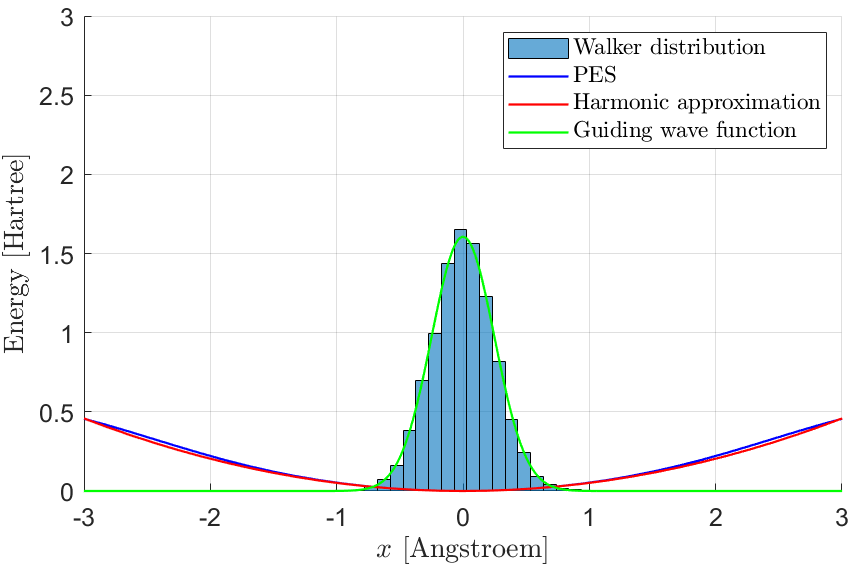
\includegraphics[width=\linewidth]{walkers1.png} 
\caption{Dimension 7}
\label{dim7}
\end{subfigure}
\begin{subfigure}{0.5\textwidth}
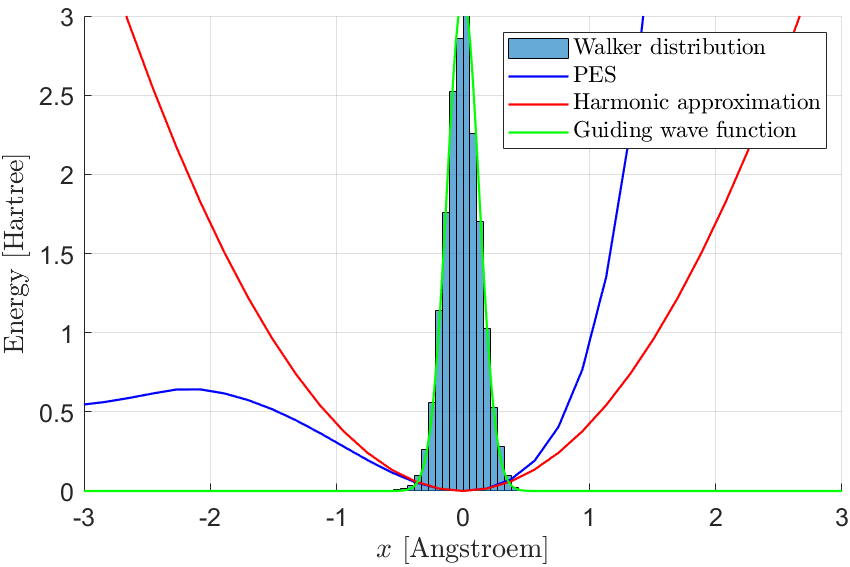
\includegraphics[width=\linewidth]{walkers2.png}
\caption{Dimension 18}
\label{dim16}
\end{subfigure}
\caption{Comparison between the PES and the harmonic approximation for two example dimensions shows a good agreement in the desired region around the minimum energy position. The calculated guiding wave function shows excellent agreement with the distribution of the walkers from an unguided DQMC simulation.}
\label{trialwf}
\end{figure}
Next, we can check the harmonic approximation by comparing it to the true PES and calculate the guiding wave function. For the ethane molecule, the harmonic approximation gives a ZPE of $0.07264$ Hartree. With the guiding wave function calculated, we can start the main calculation of the ZPE. We start with 10 parallel simulations of 1000 walkers and simulate 10000 time steps of the size $\Delta \tau = 5 \cdot 10^{-4}$ with a damping parameter $\zeta = 0.01$ Hartree. After running an unguided simulation, we see that the walkers are distributed according to the guiding wave function. Because the harmonic approximation is very good in this example, we expect the distribution of walkers to match the guiding wave function. 

\begin{figure}[h!]
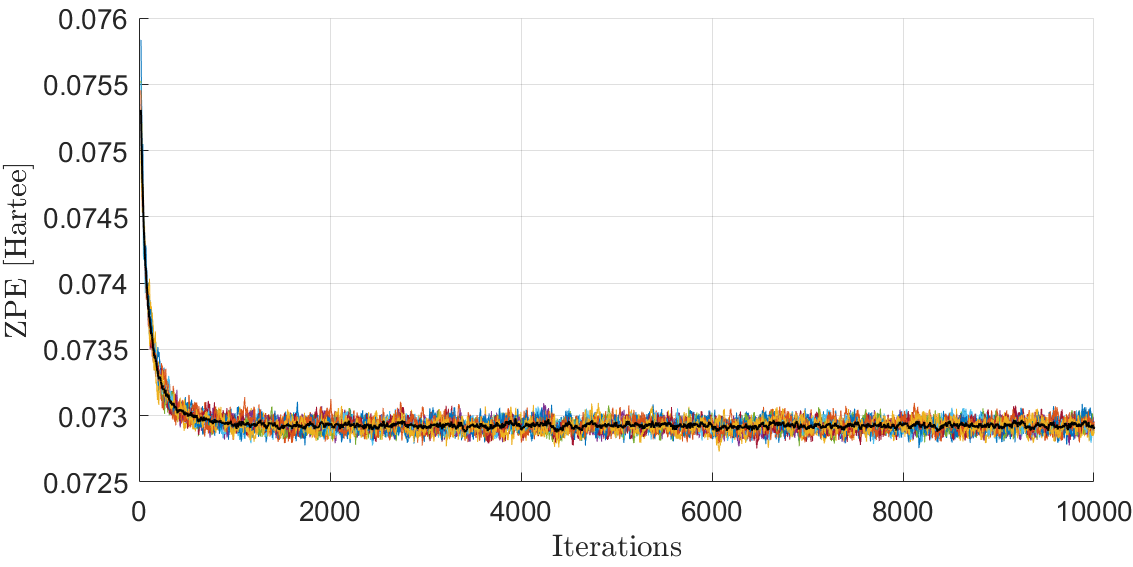
\includegraphics[width=\linewidth] {c2h6_1.png}
\caption{Evolution of the ZPE with time for the 10 different runs (in color) and the average over all the runs (in black)} \label{c2h6_1}
\end{figure}
In figure \ref{c2h6_1} we can see that the ZPE stays approximately constant after $2000$ time steps. Therefore, we can say that the system has equilibrated after $2000$ steps and we can start taking the average from there to the end of the simulation. This gives a value of $0.07293$ Hartree with a statistical uncertainty  of $2.4 \cdot 10^{-5}$ Hartree. We must keep in mind that DFTB+ is an approximate DFT method, so the result still lacks accuracy compared to a calculation with DFT energy calculations. We finally observe, that the harmonic approximation of $0.072641$ Hartree is fairly close to the DQMC result, which makes sense considering the good quality of the harmonic approximation in \ref{trialwf}. From the literature \cite{c2h6} we get a value of $0.07393$ Hartree and from the CCCBDB \cite{cccbdb} we get values forms $0.07$ to $0.08$ Hartree, depending on the method and basis set used and an experimental value of $0.072234$ Hartree (from fundamental vibrations). Even though these values are obtained from different methods, it suggests that our method is working correctly.\\
One run of 1000 walkers for 10000 time steps took 12 hours and 24 minutes on a 20-core CPU on the sciCORE scientific computing center at the University of Basel \cite{http://scicore.unibas.ch/}. Over the 10000 steps, the number of walkers remained constant at 1000 walkers.  We also observe an acceptance rate of the metropolis step of around 85\%, so we can easily calculate that we needed around 8.5 million energy calculations which means that the average energy calculation takes about 5.3 ms. With this value, one can easily predict, how long any run will take. 

\begin{figure}[h!]
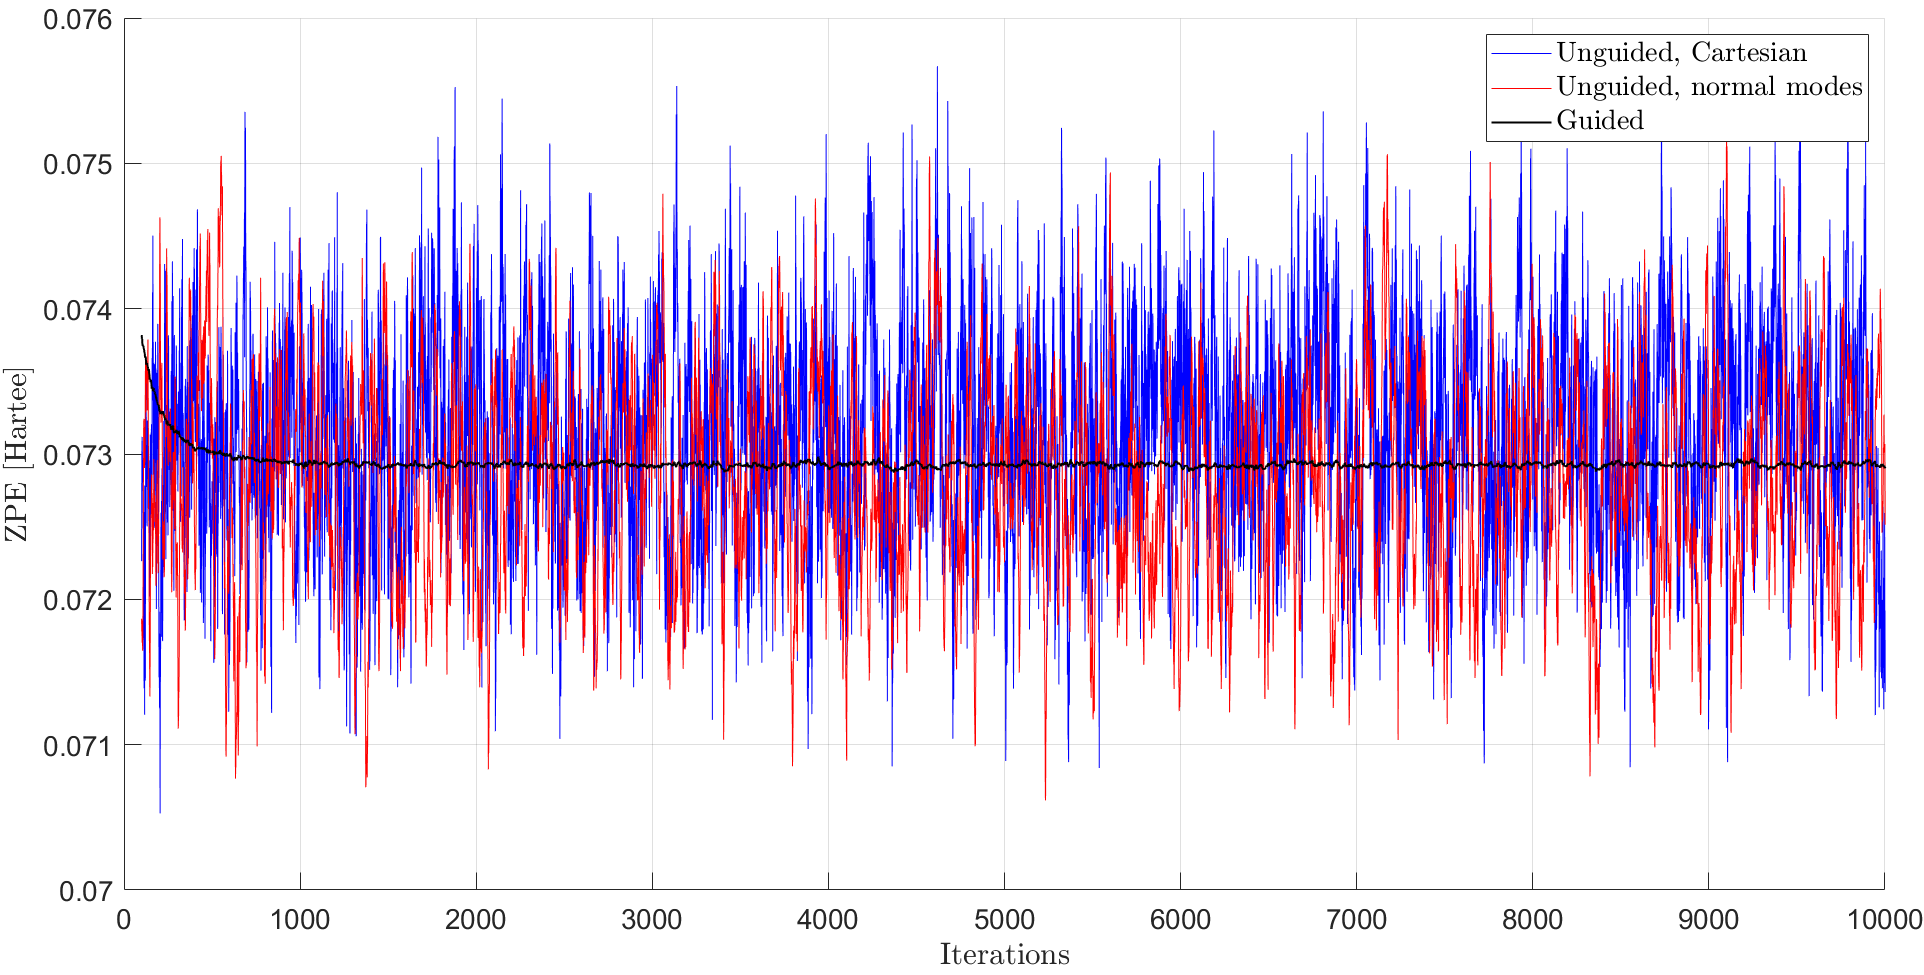
\includegraphics[width=\linewidth] {c2h6_2.png}
\caption{Comparison between guided and unguided DQMC for Cartesian and normal mode coordinates.} \label{c2h6_2}
\end{figure}
We can also compare our results with the unguided DQMC algorithm as described in \ref{uDQMC}. If we perform the calculation in Cartesian coordinates, we get a ZPE of $0.07322$ Hartree with an uncertainty of $0.00076$ Hartree and if we do the calculation in the coordinate system of the normal modes we get a ZPE of $0.07288$ Hartree with an uncertainty of $0.00062$ Hartree. Because the results are within each others uncertainties, we can conclude that both coordinate systems are equivalent in their DQMC result. The difference between guided and unguided DQMC in very noticeable. For the exact same parameters we get about 30 to 40 times less statistical uncertainty with guided DQMC. Equivalently, one would need less than 2000 steps with guided DQMC to get the same uncertainty as with unguided DQMC for the full 10000 steps.

\begin{table}[h]
\centering
 \begin{tabular}{||c | c | c||} 
 \hline
 Method & $\overline{ZPE}$ [Hartree] & $\Delta ZPE$ [Hartree] \\ [0.5ex] 
 \hline\hline
 Harmonic approximation & $0.07264$ & \\
 \hline
 Unguided, Cartesian & $0.07322$ &  $0.00076$\\
  \hline
 Unguided, normal modes & $0.07288$ &  $0.00062$\\
 \hline
 Guided & $0.07293$ & $0.00002$ \\
 \hline
 Literature value \cite{c2h6} & $0.07393$ &\\
 \hline
 CCCBDB experimental \cite{cccbdb} & $0.07223$ & \\
 \hline
 CCCBDB calculated \cite{cccbdb} & $0.07 - 0.08$ & \\
 \hline
\end{tabular}
\caption{Summary of the results for the ethane molecule and literature values for comparison.}
\end{table}
For the ethane molecule, the DQMC result  changes the harmonic approximation by less than one percent. Therefore, it does not make much sense to run a long DQMC simulation to improve the accuracy of the ZPE compared to just taking the harmonic approximation.
\newpage

\section{Buckminsterfullerene}
Due to the number of atoms, the Buckminsterfullerene ($C_{60}$) poses a bigger challenge to the algorithm. We start again by looking at the harmonic approximation and find that it matches quite very well again. Visualizing the vibrations, we find that the modes with small frequencies correspond to bending and stretching movements of the entire molecule, while the modes with large frequencies correspond to stretching and compressing the bonds between the atoms. 
Similar to the ethane molecule, the harmonic approximation works well in all the $176$ dimensions of the coordinate system of the normal modes and we get a harmonic approximation of the energy of $0.381769$ Hartree.

\begin{figure}[H]
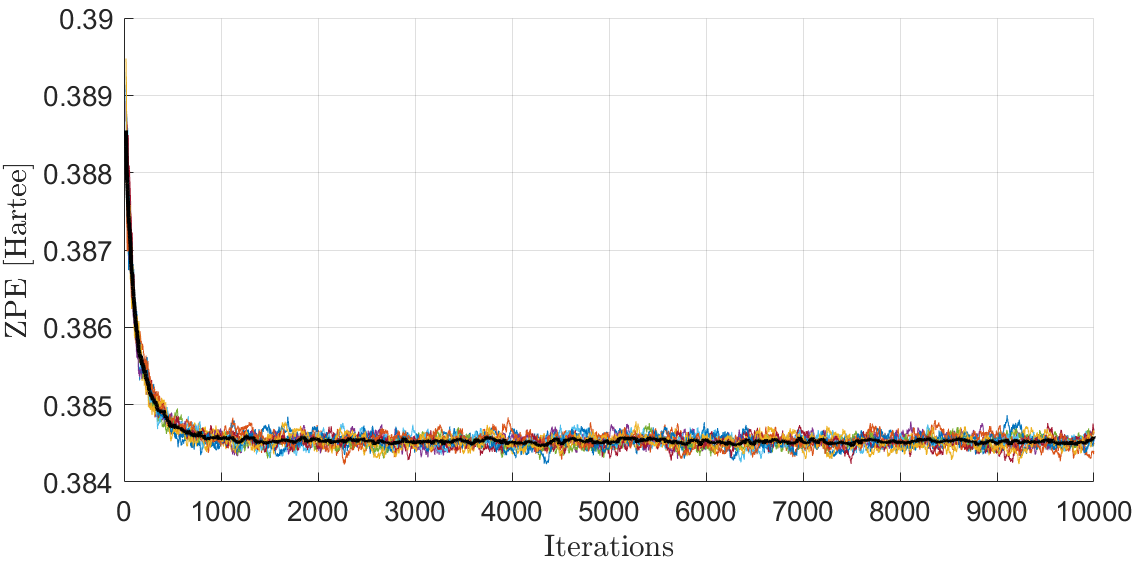
\includegraphics[width=\linewidth] {c60_1.png}
\caption{Evolution of the ZPE with time for the 10 different runs (in color) and the average over all the runs (in black). The parameters are exactly the same as for the $C_2H_6$.} \label{c60_1}
\end{figure}

We can see that the DQMC algorithm has about the same converge behavior for the $C_{60}$ than for the $C_2H_6$ but the fluctuations are about 5 times larger and the energy fluctuates with a larger frequency. Again taking averages after $2000$ simulation steps, we get a ZPE of $0.384524$ Hartree with a statistical uncertainty of $1.4 \cdot 10^{-5}$. This shows the most powerful aspect of the DQMC algorithm. The convergence does not get worse with larger systems and the accuracy only decreases slightly. For comparison, we look again at the CCCBDB \cite{cccbdb}, where we find an experimental value of  $0.369493$ Hartree and calcuated values ranging from 0.35 to 0.40 Hartree.\\
The unguided DQMC algorithm does not work well at all for the $C_{60}$. The energy rises at the start of the simulation to about 0.6 Hartree and only decreases very  slowly making it very inefficient and not worth the computer time.
\newpage

\section{Endohedral Hydrogen Fullerene}
Up to now, we have calculated the ZPE for two molecules, where the harmonic approximation worked very well. This is not the case for the endohedral hydrogen fullerene $H_2@C_{60}$\cite{h2@c60,h2@c60_anharmonic}, a system with a $H_2$ molecule trapped in the $C_{60}$ Buckminsterfullerene. In this structure, the $H_2$ experiences an anharmonic potential from the surrounding $C_{60}$. By visualizing the vibrations, we discover that for the five modes with the lowest vibrational frequency, the $H_2$ molecules rotates and translates inside the $C_{60}$ with the $C_{60}$ doing only small movements. In the other vibrational modes, the $H_2$ remains still while the $C_{60}$ vibrates similar to when we only study the $C_{60}$.\\
\begin{figure}[H]
\begin{subfigure}{0.5\textwidth}
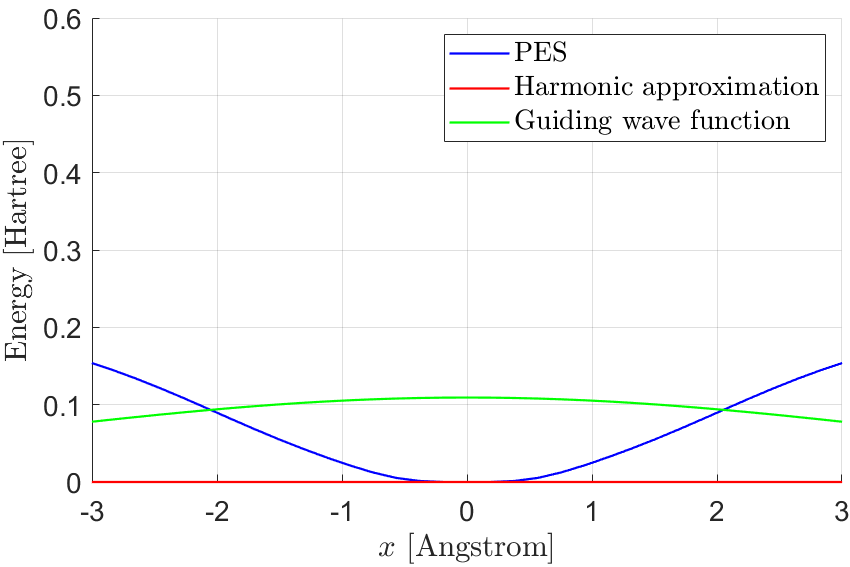
\includegraphics[width=\linewidth]{walkers4.png} 
\caption{Dimension 1}
\label{dim1}
\end{subfigure}
\begin{subfigure}{0.5\textwidth}
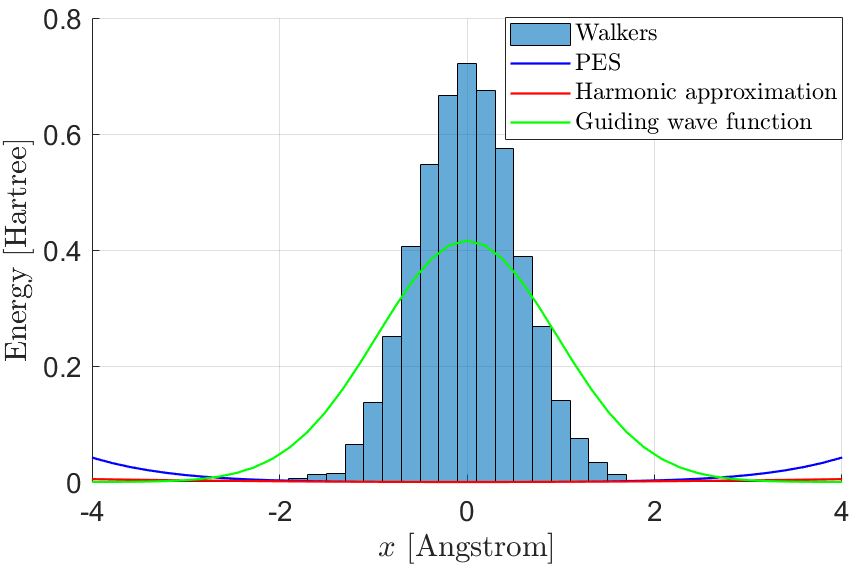
\includegraphics[width=\linewidth]{walkers3.png}
\caption{Dimension 5}
\label{dim5}
\end{subfigure}
\caption{Comparison between the PES and the harmonic approximation for two example problematic dimensions. In both cases the harmonic approximation is too flat compared to the PES. The guiding wave functions are also not good. The distribution of the walkers at the end of the simulation not distributed as the trial wave function squared but as the mixture $\psi(\bm{x})\psi_T(\bm{x})$ es discussed in \ref{init}.}
\label{trialwf}
\end{figure}
These five mentioned dimensions cause problems for the algorithm, as the potential is not harmonic. Nevertheless, we still get a guiding wave function that does not look completely unreasonable and we run the algorithm with the same parameters as before.
\begin{figure}[H]
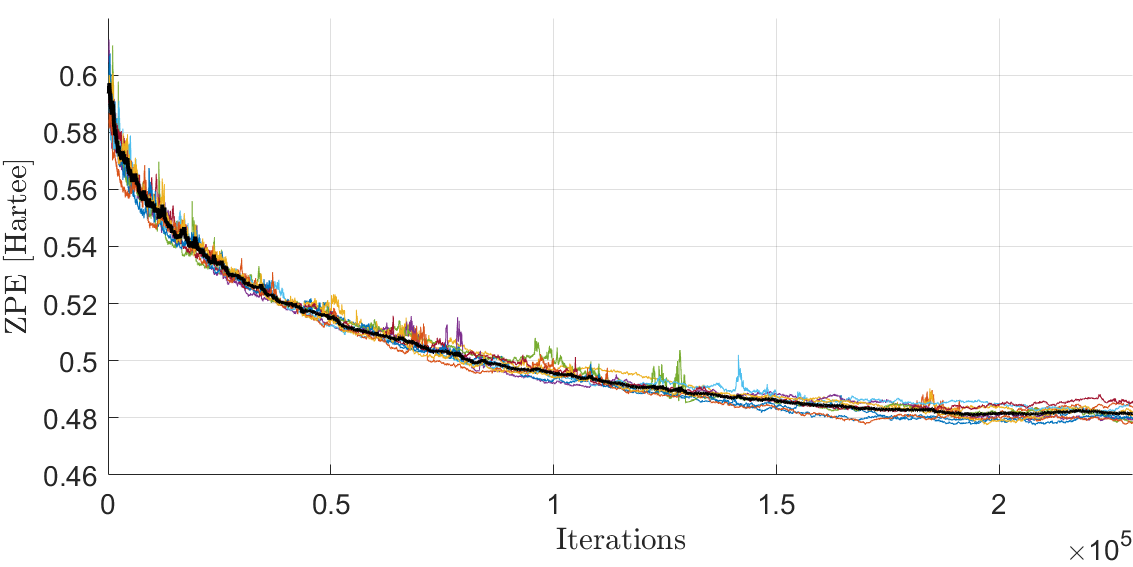
\includegraphics[width=\linewidth] {h2@c60_1.png}
\caption{Evolution of the ZPE with time for the 10 different runs (in color) and the average over all the runs (in black). The parameters are exactly the same as for the $C_2H_6$ and $C_{60}$.} \label{h2@c60_1}
\end{figure}
The convergence is much worse than for the previous two system. The $H_2@C_{60}$ system needs about 20 times more Iteration to converge due to the bad harmonic approximation and the resulting bad guiding wave function. Nevertheless, we still get a converged result, albeit with a much higher statistical uncertainty. Taking averages after $2 \cdot 10^5$ iterations we get a ZPE of 0.4818 Hartree with a statistical uncertainty of 0.0018 Hartree. For comparison, the harmonic approximation gives a ZPE of 0.3984, which is about what we would expect if we look at the $C_{60}$ and the $H_2$ separately and add their ZPEs. This result shows, that for system where the harmonic approximation fails, we can no longer use the harmonically approximated ZPE to get accurate energies as in the case of the $H_2@C_{60}$, the ZPE calculated with guided DQMC is about 21\% higher than the harmonic approximation. It further shows that the interaction between the $C$ and $H$ atoms play a large role in the characteristics of the $H_2@C_{60}$ system and that we cannot just threat them separately.
\begin{figure}[H]
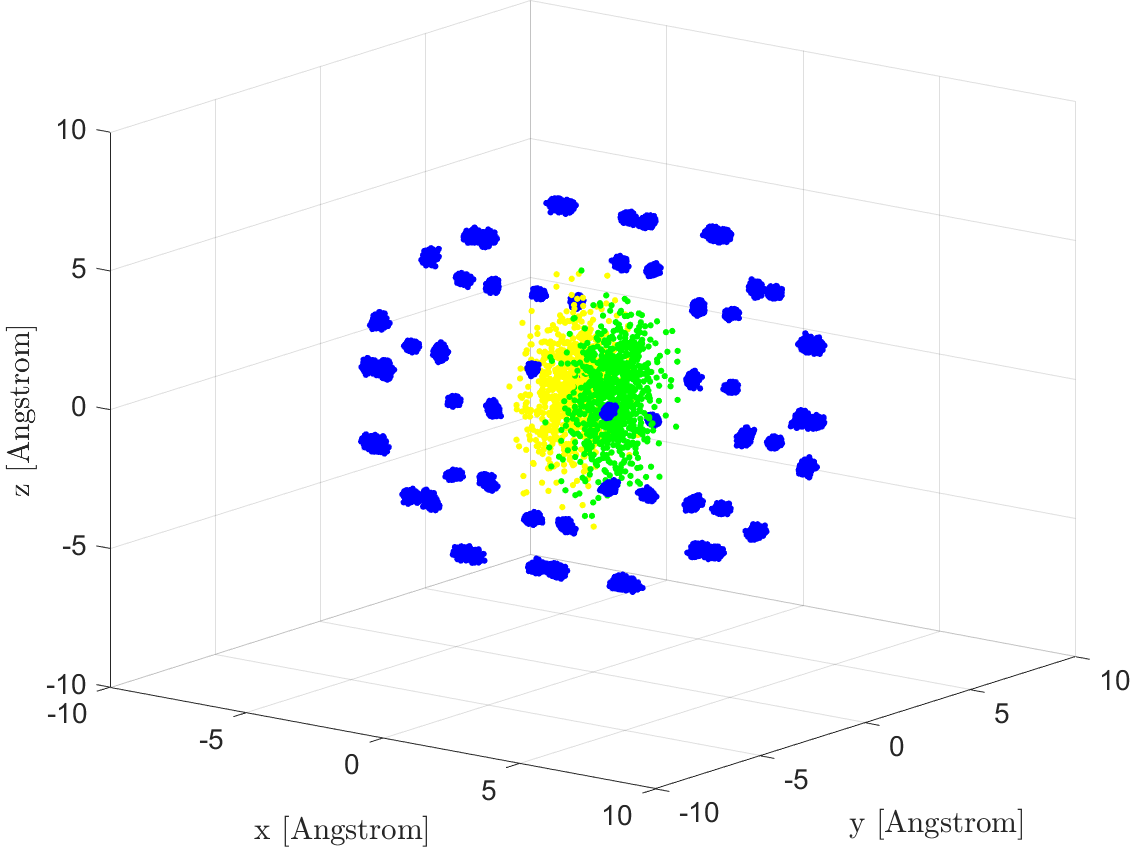
\includegraphics[width=\linewidth] {h2@c60_2.png}
\caption{Final walker positons of one run. The $C$ atoms are in blue and the left and right $H$ atoms in yellow and green.} \label{h2@c60_2}
\end{figure}
From figure \ref{h2@c60_2}, we observe that the $C$ atoms remain very localized in the $C_{60}$ cluster but the lighter $H$ atoms move around much more. Nevertheless, the left and right $H$ atoms have not managed to switch places yet. We suspect that this might be possible if we let the simulation run longer.


\chapter{Conclusion and Outlook}
We have developed a very stable and versatile diffusion quantum Monte Carlo algorithm with Gaussian guiding wave function that can be used to accurately determine zero-point energies of different molecules. For the cases of ethane and the Buckminsterfullerene we have demonstrated, that the developed algorithm converges very fast and gives reliably ZPEs with low statistical uncertainties. In these two cases, the harmonic approximation works well and gives a good guiding wave function which leads to a fast convergence. This lets us conclude that the DQMC algorithm converges equally fast, independent of the number of atoms and the only difference in running time is due to the energy calculations taking longer for larger systems. \\
On the other hand, for systems like $H_2@C_{60}$, where anharmonic effects play a big role, the convergence is much slower and the result has a larger statistical uncertainty. Nevertheless, the algorithm still converges and with the result we can show that the harmonic approximation underestimates the ZPE by around 21\%. This shows that the developed algorithm can deal with systems where the harmonic approximation fails, but at the cost of much slower convergence.\\

The goal of the Goedecker group is now to adapt the algorithm to periodic structures and calculuate the ZPE of molecular crystals, where anharmonic effects could play a big role in the ZPE. The code for the entire project is freely available on GitHub\cite{git}.

\begin{appendices}
\chapter{The Box-Muller Algorithm} \label{appendixA}
The Box-Muller algorithm transforms two $\mathcal{U}([0,1])$ random numbers ($u_1, u_2$) to two $\mathcal{N}(0,1)$ random numbers ($x_1, x_2$).

\begin{algorithm}
\caption{Box-Muller Algorithm}\label{box-muller}
\begin{algorithmic}[1]
\Procedure{BoxMuller}{$u_1, u_2$}
\State $x_1 = sqrt(-2\log(u_1))\cos(2\pi u_2)$
\State $x_2 = sqrt(-2\log(u_1))\sin(2\pi u_2)$
\EndProcedure
\end{algorithmic}
\end{algorithm}

\chapter{The Metropolis Algorithm} \label{appendixB}
The Metropolis algorithm generates random numbers distributed according to a (high-dimensional) probability distribution $p(\bm{x})$ using a Markov Chain. A Metropolis step generates a new random number $\bm{x}_{i+1}$ from a given $\bm{x}_i$ that follows the probability distribution $p(\bm{x})$. It can also be used as the accept-reject step after the move of a walker. In this case, $f$ describes the propagation of the walker according to \eqref{eq:2.10} and $\alpha$ becomes the acceptance probability \eqref{Pacc}.

\begin{algorithm}
\caption{Metropolis Step}\label{metropolis}
\begin{algorithmic}[1]
\Procedure{Metropolis}{$\bm{x}_i$}
\State $\bm{x}' = f(\bm{x}_i,$"noise"$)$ \Comment{proposing a new random number}
\State $\alpha = \frac{p(\bm{x}')}{p(\bm{x}_i)}$
\If{$\alpha \geq 1$}
	\State $\bm{x}_{i+1} = \bm{x}'$ \Comment{Accepting the proposed number}
\Else
	\State \textbf{draw} $u \sim \mathcal{U}([0,1])$
	\If{$u < \alpha$}
		\State $\bm{x}_{i+1} = \bm{x}'$ \Comment{Accepting the proposed number}
	\Else
		\State $\bm{x}_{i+1} = \bm{x}_i$ \Comment{Rejecting the proposed number}
	\EndIf
\EndIf 
\EndProcedure
\end{algorithmic}
\end{algorithm}

\chapter{Numerical Derrivatives for $E_L(x)$, $v(x)$ and the Hessian Matrix} \label{appendixC}
For a guiding wave function $\psi(\bm{x})$ the first derivative used for the drift velocity $\bm{v}(\bm{x})$ is given by
\begin{equation}
\psi'(\bm{x}_i) \approx \frac{\psi(\bm{x}_i + h) - \psi(\bm{x}_i - h)}{2h},
\end{equation}
and the second derivative used for the local energy $E_L(\bm{x})$ is given by
\begin{equation}
\psi''(\bm{x}_i) \approx \frac{\psi(\bm{x}_i + h) - 2 \psi(\bm{x}_i) + \psi(\bm{x}_i - h)}{h^2},
\end{equation}
where $h$ has to be chosen sufficiently small.
The Hessian can most efficiently be calculated by taking the derivatives of the forces
\begin{equation}
H(i,j) = \frac{\bm{f}_i(\bm{x}^{(j+)}) - \bm{f}_i(\bm{x}^{(j-)})}{2h} \mbox{\quad for all \:} i,
\end{equation}
where $\bm{x}^{(j+)}$ is the vector $\bm{x}$ with the $j$-th element increased by $h$ and $\bm{x}^{(j-)}$ is the vector $\bm{x}$ with the $j$-th element decreased by $h$.
\chapter{Gradient Descent} \label{gradient_descent}
The gradient descent algorithm takes an input configuration $\bm{x}$ with the forces $\bm{f}$ and optimizes it with respect to the minimal energy $E_{min}$. There is a lot of freedom in the choice of the parameters that we will not discuss here. The here given algorithm gives some reasonable choices for the parameters. The idea of the gradient descent is to move along the negative gradient or forces to a region where the forces and the energy are lower. The step size $\alpha$ is adjusted depending on the angle between the current forces and the previous iteration. This way the step size increases if we have consecutive moves in the same direction and decreases if we start moving in an opposite direction. 
\begin{algorithm}
\caption{Gradient Descent}\label{grad_desc}
\begin{algorithmic}[1]
\Procedure{GradientDescent}{$\bm{x}, \bm{f}, E_{min}$} \Comment{calculate the energy and forces of a given configuration}
\State $\alpha = 10^{-3}$
\State call energyandforces($\bm{x}, \bm{f}, E_{min}$)
\While{$(||\bm{f}||/N_{at} > 10^{-6})$} \Comment{iterate up to a desired precision}
	\State $\bm{f}_{prev} = \bm{f}$	
	\State $\bm{x} = \bm{x} + \alpha \bm{f}$
	\State call energyandforces($\bm{x}, \bm{f}, E_{min}$)
	\State $\beta = \arccos{(<\bm{f},\bm{f_{prev}}>/\sqrt{||\bm{f}||\:||\bm{f}_{prev}||})}$ 
	\If{$(\beta/N_{at} > 1.0472)$} \Comment{60 degree in radians}
		\State $\alpha = \alpha/2$
	\Else
		\State $\alpha = 1.05\ \alpha$
	\EndIf
\EndWhile
\EndProcedure
\end{algorithmic}
\end{algorithm}

\chapter{Input and Output Files} \label{inout}
The DQMC program requires the following input files:
\begin{itemize}
\item \textbf{geometry.xyz} describes the initial positions of the atoms in the standard .xyz file format. The first line contains the number of atoms $N_{at}$. The second line can be used for comments and will not be read. Starting on the third line are the $N_{at}$ atoms, one in each line with their atomic symbols and then their x, y, and z coordinates. The position coordinates must be in units of Angstrom.
\item \textbf{masses.in} contains the masses of the atoms. The first line contains again the number of atoms and the following lines contain the masses in atomic mass units in the same order as the atoms in \textbf{geometry.xyz}.
\item \textbf{dqmc.in} is the input file for the parameters of the DQMC calculation. It contains the following lines:\\
\verb+damping 0.01d0 #damping constant+\\
\verb+no_walkers_start 10000 #initial number of walkers+\\
\verb+delta_t 5.d-4 #discrete time step+\\
\verb+n_steps 10000 #number of simulation steps+\\
\verb+debug_extended .FALSE. #show extended information+\\
\verb+continue_run .FALSE. #continue a previous simulation+\\
\verb+grad_descent .TRUE. #do a gradient descent+\\
\\
If \verb+continue_run+ is set to true, the files \textbf{et\_noWalkers\_e0.out} and \textbf{walker\_positions.out} from the simulation that wants to be continued are also required as input files. The simulation then continues from where it had finished for \verb+n_steps+ more steps. In the output file \textbf{et\_noWalkers\_e0.out} the new steps will be added to the end of the file.
\end{itemize}
If the simulation is run using DFTB+, the input files such as \textbf{dftb\_in.hsd} and the Slater-Koster files are also required. Details can be found in the DFTB+ manual\cite{dftbp_manual}.\\

The DQMC program gives the following output files:
\begin{itemize}
\item \textbf{et\_noWalkers\_e0.out} contains the trial energy $E_T$, the number of walkers $N_w$ and the current ground state estimate $E_0$ in its columns for each iteration. The energies are given in the Hartree energy unit.
\item \textbf{walker\_positions.out} contains the displacements of the walkers in the coordinate system of the normal modes at the end of the simulation. The values are all in one column starting with the $N_{at}-6$ values for the first walker.
\item \textbf{walker\_positions\_cartesian.out} contains the final positions of the walkers in Cartesian coordinates in the .xyz format (without the first two lines, the atomic symbol, but in the same order as in \textbf{geometry.xyz}).
\item \textbf{energies\_weights.out} contains the local energy $E_L$ in column one and the weight $w$ in column two for all the walkers.
\item \textbf{eigenvalues.out} contains the eigenvalues of the Hessian matrix in ascending order. This order also corresponds to the order of the displacements in \textbf{walker\_positions.out}.
\item \textbf{modes.txt} can be directly loaded into the PyMol plugin PyVibMS \cite{PyVibMS} together with \textbf{geometry.xyz} to visualize the vibrational modes.
\end{itemize}

\end{appendices}

\bibliographystyle{unsrt}
\bibliography{references}

\end{document}